\subsection*{Separate migration, execution and scientific axes}
\begin{longtable}{p{0.25\linewidth}p{0.68\linewidth}}\toprule Axis & Actual status\\\midrule
migration\_\allowbreak{}gate & PASS\_\allowbreak{}GEOMETRY\_\allowbreak{}ADAPTER \\
execution\_\allowbreak{}gate & PASS\_\allowbreak{}BOUNDED\_\allowbreak{}GEOMETRY\_\allowbreak{}SMOKE \\
scientific\_\allowbreak{}gate & UNRESOLVED\_\allowbreak{}MISSING\_\allowbreak{}PHYSICAL\_\allowbreak{}INPUTS \\
scientific\_\allowbreak{}status\_\allowbreak{}promoted & False \\
\bottomrule\end{longtable}
\subsection*{Measured geometry and resolution sensitivity}
\begin{longtable}{p{0.15\linewidth}rrrr}\toprule Topology & N & Native length & Mean curvature & Midpoint writhe\\\midrule
0\_1 & 64 & 12.52869104 & 0.5033844161 & 0 \\
0\_1 & 128 & 12.54017859 & 0.6604430041 & 0 \\
3\_1 & 64 & 16.32543462 & 0.9829584087 & 3.412398906 \\
3\_1 & 128 & 16.36257488 & 1.034079532 & 3.408273635 \\
4\_1 & 64 & 22.35286777 & 0.910604241 & 0.2068828022 \\
4\_1 & 128 & 22.44280283 & 0.9558892656 & 0.2007498053 \\
\bottomrule\end{longtable}
Two registered levels expose sensitivity; they do not establish convergence or physical calibration.
\begin{figure}[htbp]\centering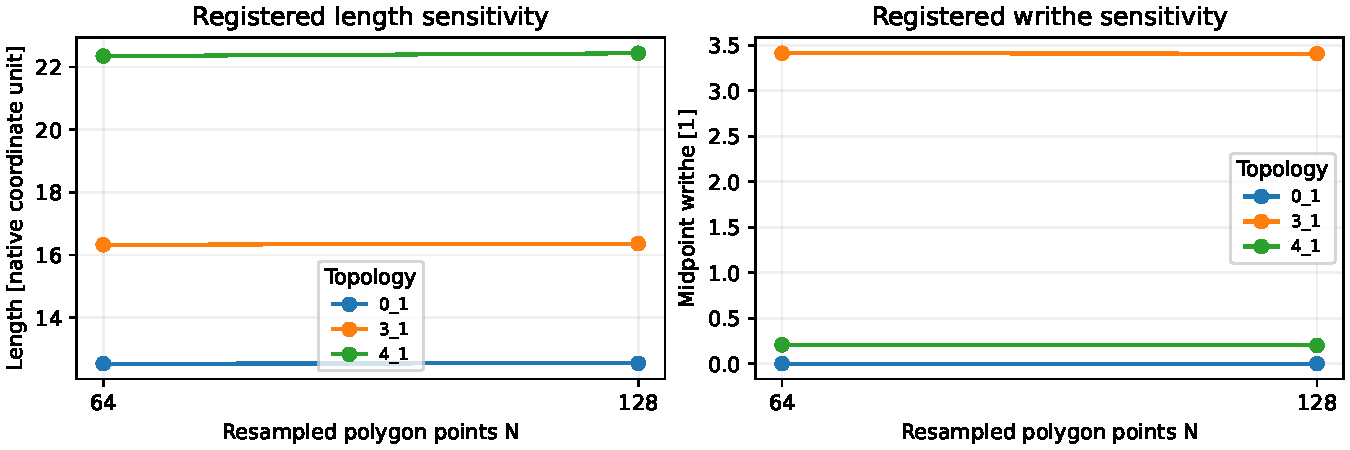
\includegraphics[width=\linewidth]{figures/geometry_sensitivity.pdf}\caption{Actual N=64 and N=128 measurements from PLOT\_DATA.json. Native lengths have no calibrated SI scale; writhe is dimensionless. No fitted trend or continuum extrapolation.}\end{figure}
\subsection*{Actual native/reference comparisons}
\begin{longtable}{p{0.15\linewidth}rrrr}\toprule Carrier topology & N & Velocity max abs & Writhe abs & Distance abs\\\midrule
0\_1 & 64 & 2.7756e-17 & 0 & 0 \\
0\_1 & 128 & 6.9389e-18 & 0 & 0 \\
3\_1 & 64 & 5.5511e-17 & 0 & 0 \\
3\_1 & 128 & 5.5511e-17 & 0 & 0 \\
4\_1 & 64 & 2.2204e-16 & 0 & 0 \\
4\_1 & 128 & 2.2204e-16 & 0 & 0 \\
\bottomrule\end{longtable}
\subsection*{Exact gate execution and claim authority}
\begin{longtable}{p{0.08\linewidth}p{0.28\linewidth}p{0.34\linewidth}p{0.19\linewidth}}\toprule Gate & Execution & Qualification & Allows dependent claim\\\midrule
G0 & EXECUTED & QUALIFIED & True \\
G1 & EXECUTED & QUALIFIED & True \\
G2 & EXECUTED & QUALIFIED & True \\
G3 & NOT\_\allowbreak{}EXECUTED & BLOCKED\_\allowbreak{}PREREQUISITE & False \\
G4 & NOT\_\allowbreak{}EXECUTED & BLOCKED\_\allowbreak{}PREREQUISITE & False \\
G5 & EXECUTED & DIAGNOSTIC\_\allowbreak{}ONLY & False \\
G6 & DISABLED & NOT\_\allowbreak{}APPLICABLE & False \\
G7 & NOT\_\allowbreak{}EXECUTED & BLOCKED\_\allowbreak{}PREREQUISITE & False \\
G8 & NOT\_\allowbreak{}EXECUTED & BLOCKED\_\allowbreak{}PREREQUISITE & False \\
G9 & DEFERRED & DEFERRED & False \\
\bottomrule\end{longtable}
\subsection*{Missing scientific evidence}
\begin{itemize}
\item Calibrated physical length and SI source scale
\item Independent physical energy spectrum/gaps and relaxation/couplings
\item Independent thermodynamic sampled state counts
\item Held-out force/pressure and mechanism validation
\item Spatial/time/solver/regularization convergence beyond this two-level geometry smoke
\end{itemize}
